
\subsection{CLU}
\label{sec:algorithms:clu}

CLU, short for Co-Optimizing Locality and Utility, was presented in 2014.
The authors of CLU recognize that recent research in LLC partitioning has followed two distinct directions.
Some publications optimize for access locality and attempt to improve performance by changing the lifetime of blocks in LRU managed caches.
DIP, TADIP, and NUCache are three such solutions that use novel methods to reduce or extend the lifetime of blocks in an elsewise LRU managed cache.
Other publications recognize the usefulness of utility and do way-partitioning between cores based on their utility values.
Examples here are UCP and PIPP.
Both UCP and PIPP are forced to use LRU as the underlying algorithm because they both depend on the stack property of LRU to do utility calculations~\cite{Qureshi2006, Xie2009}.

The authors of CLU present a novel approach for calculating the utility curve of a BIP managed cache.
BIP, as covered earlier, is one of the two insertion policies under DIP and TADIP. 
BIP violates the stack property of LRU by mostly inserting new rows at the MRU position, or at a low probability in LRU position.
To correctly measure the utility curve of a BIP managed k-way cache, one needs k ATDs; ATD($1$), ATD($2$), ... ATD($k$). 
Where ATD($x$) is an x-way ATD.
In contrast, the utility curve of an LRU managed cache can be found using one ATD, due to the stack property.
Having k ATDs per core sharing the LLC is not a realistic goal due to the required overhead.
The authors of CLU propose a simplification where there are $m = log_2 k$ ATDs; ATD($1$), ATD($2^1$), ..., ATD($2^m$).
A linear increase between the sample points is assumed when calculating the final utility curve.
It should be noted that the storage overhead of m ATDs in total is less than twice the overhead of the single ATD($k$) required to sample the LRU curve.

CLU uses the two curves first to allocate ways to each core using the same algorithm as shown for UCP in section~\ref{sec:algorithms:ucp}.
The only difference is that the algorithm uses either the LRU or BIP value when estimating utility given an allocation, depending on which algorithm performs best.
During runtime, CLU works like UCP.
The only exception is that the core's ways are managed by either LRU or BIP, depending on which algorithm has the best utility value for the number of ways currently assigned to that core.

Figure~\ref{fig:algorithms:clu_example} is an example LIP and BIP utility plot for a core sharing a 16-way cache.
For each way value, the maximum achievable utility is the maximum of the LIP and BIP line.
Hence, when the lookahead algorithm is used to assign ways to each core, the maximum of the LIP and BIP value is used.
If the sample core were assigned 2 ways it would use BIP replacement, this follows from the fact that BIP has a higher utility at 2 ways.
However, if the core were assigned 12 ways, it would use LIP replacement because LIP has a higher utility at that point.

\begin{figure}[ht]
    \centering
    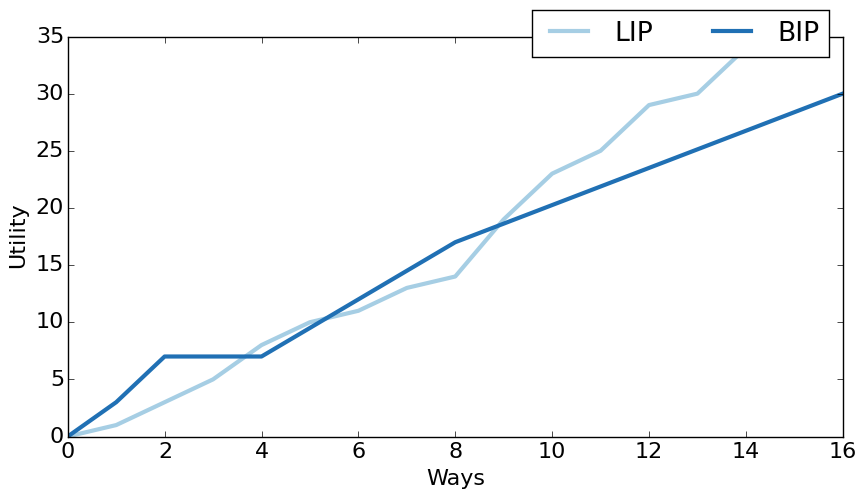
\includegraphics[width=.65\textwidth]{figures/algorithms/clu-utility}
    \caption{Utility plot of BIP and LIP for a 16-way cache.}
    \label{fig:algorithms:clu_example}
\end{figure}
